\chapter{Introduction}\label{chap:introduction}

\epigraph{\emph{A program that is used and that, as an implementation of its specification, reflects some other reality, undergoes continuous change or becomes progressively less useful.
The change or decay process continues until it is judged more cost effective to replace the program with a recreated version.}}{--- Meir Lehman}

%\section{The relentless endeavor of software craftmanship}
\lettrine{T}{he} opening quote of this chapter is the first of the five laws of software evolution formulated by Lehman in the late 1970's \cite{Lehman1979}.
The law refers to the fact that all software is designed to operate in a specific environment and to satisfy a specific set of requirements. 
However, every environment, and every requirement, is bound to change eventually, rendering the software obsolete. %, unless it changes accordingly.
Therefore, a constant need of adapting the software and keeping it \emph{relevant} for its stakeholders arises.
This continuous adaptation is a \emph{relentless endeavor} that requires an ever-increasing amount of resources and, over time, destabilises the \emph{sustainability} of a software project.

A software project is \emph{sustainable} if the project owner is capable of applying whatever valuable change they ought to make, in a timely fashion \cite{Winters2020}.
However, design decisions and implementation choices made early on in the project's lifetime inevitably affect the decisions we have to make in the present, often making them harder.
Over time, as the system grows old, our capability of adapting the software to new requirements and changes in the environment grows narrower, and making changes becomes more expensive.
Eventually, the system becomes \emph{unsustainable}: it is \emph{poorly maintainable} -- i.e. it is hard to fix bugs -- and with \emph{limited capabilities} to evolve -- i.e. it is difficult to implement new functionality. In other words, the second sentence of Lehman's first law of software evolution comes into play.

In 1992, Ward Cunningham cleverly adapted and reframed both of these concepts (sustainability and Lehman's first law) under the term \emph{technical debt} \cite{Cunningham1992}. 
Since then, technical debt has gained a lot of traction among both practitioners and researchers alike, as it concerns a problem that (almost) every non-trivial software system suffers from. 
Over the years, several studies have made great progress in identifying the causes and effects of technical debt \cite{Brown2010,Kruchten2012}.
A comparable amount of effort was also spent in designing and developing strategies and techniques to \emph{manage} TD \cite{Li2015} in order to aid decision-makers. 
Similarly, several tools were developed to automatically \emph{measure} TD using source code as input \cite{Avgeriou2021}, or \emph{track} it manually \cite{Martini2016}.

Technical debt can materialise into various forms, ranging from source code violations \cite{Letouzey2012,Curtis2012} and design-level flaws \cite{Marinescu2012} to sub-optimal decisions made at the architectural level \cite{Ernst2015,Yli-Huumo2014}. One form of such architectural decisions are architectural smells (AS); they are defined as \emph{``commonly (although not always intentionally) used architectural decisions that negatively impact system quality} \cite{Garcia2009} and have gained a lot of attention from researchers over the past years \cite{Verdecchia2018}.
AS are a particularly risky type of technical debt: they involve architecture-level artefacts, so their impact is much larger and affects software development in the long run. 
%Although existing literature has devoted a considerable amount of effort to study AS \cite{Mo2015,Le2016,Arcelli2016}, our understanding of AS is still incomplete.
%This dissertation aims at improving the current state of the art concerning our understanding of AS by answering questions such as: \emph{how are AS introduced?; how do AS evolve?; and, what is their impact on software maintenance (i.e. technical debt)?}

The fundamental proposition of this thesis is that a better understanding of AS will allow software practitioners to better manage technical debt, thus making software maintainability and evolvability more cost-effective; this can, in turn, slow down the decaying process mentioned by Lehman's first law of software evolution and defer the replacement of the software.

In the upcoming sections, we will introduce the concepts of technical debt and architectural smells in further detail, as these are the \emph{leitmotif} of this dissertation.
I will also decompose the research problem addressed in this thesis into multiple research questions and explain the methodology used to answer them.


\section{Technical Debt}
\subsection{History, definitions, and types}
In 1992, Cunningham first introduced the concept of \emph{technical debt} (TD) \cite{Cunningham1992}. 
The term was coined to indicate the necessity of releasing software that, may work perfectly, but does not meet the criteria of software that is sustainable in the long-term. 
Cunningham himself calls this an \emph{``unmasterable program''} that is \emph{``dangerous''} unless the \emph{debt} is repaid.
Unfortunately, TD repayment is not always feasible, as software practitioners have to work with limited time and budget, resulting in most of TD not being repaid \cite{Digkas2018}.
The time spent on not-quite-right code counts as \emph{interest} on that debt \cite{Cunningham1992}, making software projects more expensive to maintain, whereas the not-quite-right code itself is referred to as \emph{principal}.
Technical debt is a powerful metaphor that, essentially, conveys the importance of sustainable software -- and of Lehman's first law of software evolution -- in terms that are easy to understand and communicate to others. 


A well-accepted definition of TD is the following: 
%\emph{TD reflects the technical compromises that software practitioners make in order to achieve a short-term advantage at the expense of creating a technical context that increases complexity and cost in the long-term} 
\emph{``in software-intensive systems, technical debt is a collection of design or implementation constructs that are expedient in the short term, but set up a technical context that can make future changes more costly or impossible. Technical debt presents an actual or contingent liability whose impact is limited to internal system qualities, primarily maintainability and evolvability''}\cite{Avgeriou2016}. 
Hence, an organization can get into debt and use it as leverage to temporarily increase productivity, as long as it is aware of the debt and is planning to repay it in due time.
However, if the organization is not aware that it is accruing TD, or does not repay it on time, the amount of interest may become too high, causing the failure of the project due to the huge cost of implementing changes.

Since the original conception of the metaphor by Cunningham, it has been extended, engulfing several aspects of the software development process like architecture, design, requirements, testing and documentation \cite{Brown2010}.
The current research literature has explored the concept in breadth and depth and has proposed and analyzed multiple taxonomies and types of TD.
A common way of categorising TD is by the type of artefacts it affects. Using this approach, Li et al. \cite{Li2015} identified several different types of TD, namely \emph{Requirements TD}, \emph{Architectural TD}, \emph{Design TD}, \emph{Code TD}, \emph{Test TD}, \emph{Build TD}, \emph{Documentation TD}, \emph{Infrastructure TD}, and \emph{Versioning TD}.

In this thesis, we will mostly focus on \emph{Architectural TD} (ATD), the type of TD that affects the architecture of a software.
Examples of ATD are architectural violations (e.g. the implemented architecture is not compliant with a set of predefined architectural rules), poor application of well-known architectural patterns, early architectural decisions that had unexpected trade-offs, or architectural smells.
As aforementioned, this dissertation is centered around this last form of ATD, that is architectural smells.

\subsection{Metaphor's weaknesses and limitations}
The use of the TD metaphor to describe software issues has received some criticism from the research community too.
One of the major shortcomings of the metaphor, according to Schmid \cite{Schmid2013}, is the lack of a standard unit of measurement and the difficulty to measure it because of the fuzzy boundaries of the different TD components.
Moreover, still according to Schmid \cite{Schmid2013}, not all TD is \textit{effective} TD, but it can also be \textit{potential} TD, since it is not sure if there will be any interest to be paid on that debt.
This may be the case when some specific code will never have to be modified again, hence no interest will ever be paid on such code; as if it had no debt.
Schmid also argues that the more detailed the effect of TD taken into account, the higher its estimation gets: adding up individual contributions to TD will result in counting the same underlying cost multiple times, leading to an exaggerated value of TD \cite{Schmid2013}.

Other studies point out that the metaphor may encourage the detrimental behaviour of introducing debt thinking that a faster delivery can be achieved, without any drawbacks. This is favoured by the fact that, in some cases, the people who take the debt are not necessarily the same who pay it back \cite{Allman2012}.


\section{Architectural smells}
The term \emph{architectural smell} (AS) was initially introduced by Lippert and Roock in 2006 \cite{Lippert2006} to refer to violations of recognised design principles (such as the ones defined by Martin \cite{Martin2018}) that result in undesired dependencies, overblown size, and excessive coupling \cite{Garcia2009}.
Alternatively, architectural smells can be seen as error-prone or change-prone design spots that hinder software maintainability at an architectural level \cite{Mo2015}.
It is important to note, however, that architectural smells are an \emph{indication} that something may be problematic, but they do not necessarily result in problems.

This definition of architectural smells may sound very similar to the definition of \emph{code smells} provided by Kent Beck\footnote{Read \url{https://wiki.c2.com/?CodeSmell} for more info.}. 
However, there is a clear distinction between the two: architectural smells involve multiple classes, packages, architectural layers, or even sub-systems\footnote{From hereafter collectively referred to as \emph{elements}.} \cite{Lippert2006}, whereas code smells (CS) arise at line of code, method, or class level \cite{Fowler2002}. 
This means that architectural smells, contrary to code smells, require \emph{large refactorings} in order to be removed from a system \cite{Lippert2006}.
Therefore, given the different scope and granularity, architectural smells and code smells are considered two different categories \cite{Sharma2020}.
This difference between the two categories of smells is also supported by empirical evidence \cite{Arcelli2019}.

Architectural smells can be of different types, with each type having its own definition and implications for the maintainability and evolvability of the affected elements \cite{Azadi2019}.
An architectural smell type can have multiple instances affecting a system, with each instance having a different severity (more on this in Section \ref{c2:sec:arch-smells}).
An example of an architectural smell type is \emph{Cyclic Dependency}, which arises when a set of elements (e.g. classes, or packages) depend on each other in a cycle.

The architectural smell types that are of interest to this PhD project are \emph{Cyclic Dependency (CD), Hublike Dependency (HL), God Component (GC), and Unstable Dependency (UD)}.
In Section \ref{sec:intro:problem-statement} we elaborate on the reasons why we opted to focus on these four types of AS.
The definitions of each AS type will be given in Section \ref{c2:sec:arch-smells}.


\section{The project SDK4ED and \textsc{Arcan}}
This PhD project was conducted in the context of the SDK4ED project, a project funded by the European Union under the Horizon 2020 programme.

The vision of SDK4ED was to minimize the cost, the development time and the complexity of low-energy software development projects, by providing tools for automatic optimisation of multiple quality requirements, such as Technical debt, Energy efficiency, Dependability (i.e. Reliability, Availability, and Security) and Performance. 
One of the topics on which the project has innovated, is researching and developing tools to identify the \textit{trade-offs} between runtime and design-time software quality attributes at multiple levels of abstractions (code, design, and architecture).
In this regard, our study investigates specifically the interaction between Technical debt (i.e. Maintainability and Evolvability) and Reliability, which map to design-time and  runtime quality attributes, respectively. Further details on the project is available on its website\footnote{Browse \url{https://sdk4ed.eu/}.}.

As part of the SDK4ED project, I also contributed to the open source version of \textsc{Arcan}, a tool to automatically detect AS in a system, by adding support for Java source code, support for Git to do evolution analyses, and the detection of the God Component smell.
\textsc{Arcan} will be fully introduced in Section \ref{c2:sec:arcan}.

\section{Research design}\label{sec:intro:research-design}
\subsection{Problem statement}\label{sec:intro:problem-statement}
In this dissertation, we address the problems that practitioners face when attempting to make changes to their systems in the presence of AS; we also argue that by providing better support to target AS as part of TD management, we can help practitioners to make changes more effectively and efficiently. 
To better explain the problem, let us quickly look at the key activities of TD management \cite{Li2015}; note that we only mention the five most important and most studied activities \cite{Li2015}, and focus specifically on AS (out of all TD types).
These five activities are: (1) \emph{identify} what elements in the system are affected by AS and the type of the smells; (2) \emph{quantify} the impact of each smell on the development activities (both maintenance and evolution); (3) \emph{prioritise} the smells in order to determine the urgency to refactor; (4) \emph{repay} the debt by refactoring smells according to the prioritisation strategy adopted; and finally (5) regularly \emph{monitor} the evolution of TD and smells over time.

The current research landscape contains plenty of studies that focus on the first activity of TD management for architectural smells -- i.e.  \emph{identification} -- whereas the work done on the other activities is not as mature.
Consequently, practitioners have the means to identify the AS affecting a system, but there is limited understanding, and most importantly very little tool support, for the remaining activities.

This situation stems from the fact that early research work on architectural smells (rightfully) focused on identifying new types of smells, theoretically defining them, proposing detection rules, and finally describing their impact on software maintenance from a theoretical, and then empirical, point of view \cite{Lippert2006,Garcia2009,Mo2015,Le2016,Arcelli2016}.
Subsequently, tools for automatic detection of AS were proposed, by both academia and industry \cite{Avgeriou2021,Khomyakov2020}, and AS detection became a more feasible option for many practitioners that could not afford to do a manual assessment.
However, the rest of the activities, from quantification through monitoring, are not really supported in practice due to: a) the scarcity of research on these activities; b) the limited availability of the few research tools that focus on those specific activities; and c) the difficulty to use such tools \cite{Khomyakov2020}.
In the best case scenario, this leaves practitioners to rely on intuition and assumptions instead of \emph{data} and \emph{well-established practices}; in the worst case scenario, they do not consider AS management at all.
In the long run, both are likely to cause exceedingly high costs in order to apply any changes, thus diminishing the long-term sustainability of the system \cite{Winters2020}. 
Eventually, it becomes more convenient to rewrite the whole project \cite{Lehman1979}, or rely on a third party solution; but in some cases, neither of these options may be feasible, leading to software `bankruptcy' \cite{Ampatzoglou2015}.

This problem is summarised by the following statement:
\begin{quote}\itshape
    ``The detection of architectural smells alone is not sufficient for practitioners to take informed TD management decisions.
    Practitioners need to know the amount of TD each instance amounts to, what the available prioritisation strategies are, and the trend of the TD incurred over time. This information can help them better implement TD repayment.''
\end{quote}

To further scope down the problem, we considered the fact that dozens of architectural smells have been reported in books and scientific literature, and it would be infeasible to address all of them. Thus, we decided to focus our attention only on the four architectural smells (CD, HL, GC, UD -- see Section \ref{c2:sec:arch-smells}) that are the most prominent in the literature\cite{Azadi2019}; two of them are also well known in the industry \cite{Lippert2006,Martin2018}.
Moreover, the literature also provides manually-validated, open source tools that we can use to detect these smells.
In particular, we relied on \textsc{Arcan} \cite{Arcelli2016,Arcelli2017,Martini2018}, and through the work in this dissertation, we actively contributed to improving the tool.

\subsection{Design science as research methodology}
The research project that this dissertation is based on, adopts the design science framework, as developed by Wieringa \cite{Wieringa2014} and depicted in Figure \ref{fig:design-science}.
Design science concerns the \emph{design} and \emph{investigation} of artefacts (e.g. a software component, a method, a service, an organisation, etc.) in context \cite{Wieringa2014}.
\emph{Design} refers to allowing the design of an artefact that improves a problem context, namely, that solves a \emph{design problem}. 
\emph{Investigation} refers to allowing to answer \emph{knowledge questions} about the artefact in context.

Design problems call for a change in the real world; in contrast, knowledge questions ask for knowledge about the real world.
The distinction between design problems and knowledge questions is often confusing, as design problems can be formulated to look like knowledge questions.
Figure \ref{fig:design-science} can help us distinguish these: if the question asks  \emph{about a solution} to a problem, then it is a design problem; if it seeks knowledge \emph{about the world}, then it is a knowledge question.

A concrete example of design science is Software Engineering itself \cite{Wieringa2014}.
Software Engineering is a design science that seeks to understand and solve the problems of creating and maintaining software to achieve the stakeholders' goals.

A concrete example of a design problem is: \emph{design an approach to measure technical debt principal based on architectural smells.}
A concrete example of a knowledge question is: \emph{how accurate is such an approach?}

\begin{figure}
    \centering
    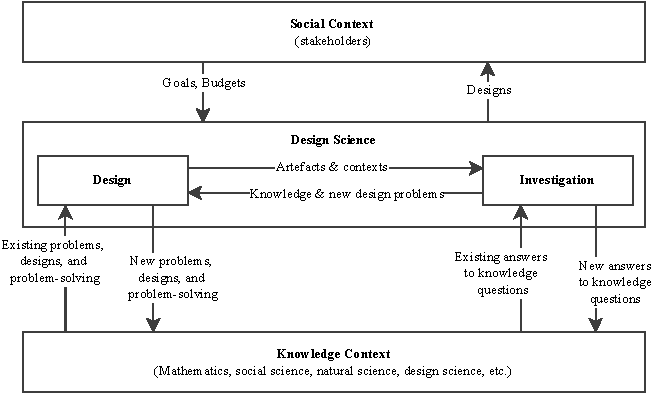
\includegraphics[width=.9\textwidth]{c1/design-science-diagram.pdf}
    \caption{The framework for design science proposed by Wieringa \cite{Wieringa2014}.}\label{fig:design-science}
\end{figure}

Design science is an iterative process where a researcher analyses a design problem, identifies a solution, evaluates the solution, and, if the solution is not satisfactory, they start over. 
The analysis of the design problem and its evaluation are referred to as design cycle.
Iterations through the design cycle may uncover aspects of the original design problem that were initially unknown.
The evaluation process also allows for additional design problems or knowledge questions to emerge.

These characteristics make the design science framework suitable for describing long-term research such as PhD projects.
Indeed, a PhD project starts with an initial design problem, which can be decomposed into new, smaller design problems and knowledge questions.
By answering the knowledge questions, the researcher can identify, with the new knowledge acquired, a solution to the design problems previously identified, which in turn might uncover new design problems and knowledge questions.
The cycle repeats until a design solution is found for the original problem.

\subsection{Problem decomposition}\label{c1:sec:problem-decomposition}
This section elaborates on how the research project presented in this thesis is framed according to the design science framework. 
Figure \ref{fig:intro:problem-decomposition} decomposes the problem statement introduced in Section \ref{sec:intro:problem-statement} into design problems and knowledge questions.
The different colors and arrows are to be read as follows: light grey boxes refer to design problems; yellow boxes refer to knowledge questions; thin arrows represent decomposition; whereas thick arrows represent sequence.
In the remainder of this section, we will use the term \emph{research question} (RQ) to refer to both design problems and knowledge questions.
Research questions are numbered to easily refer to them, and, with the exception of RQ1, are decomposed into multiple sub-RQs that are labelled with letters.

\begin{figure}
    \centering
    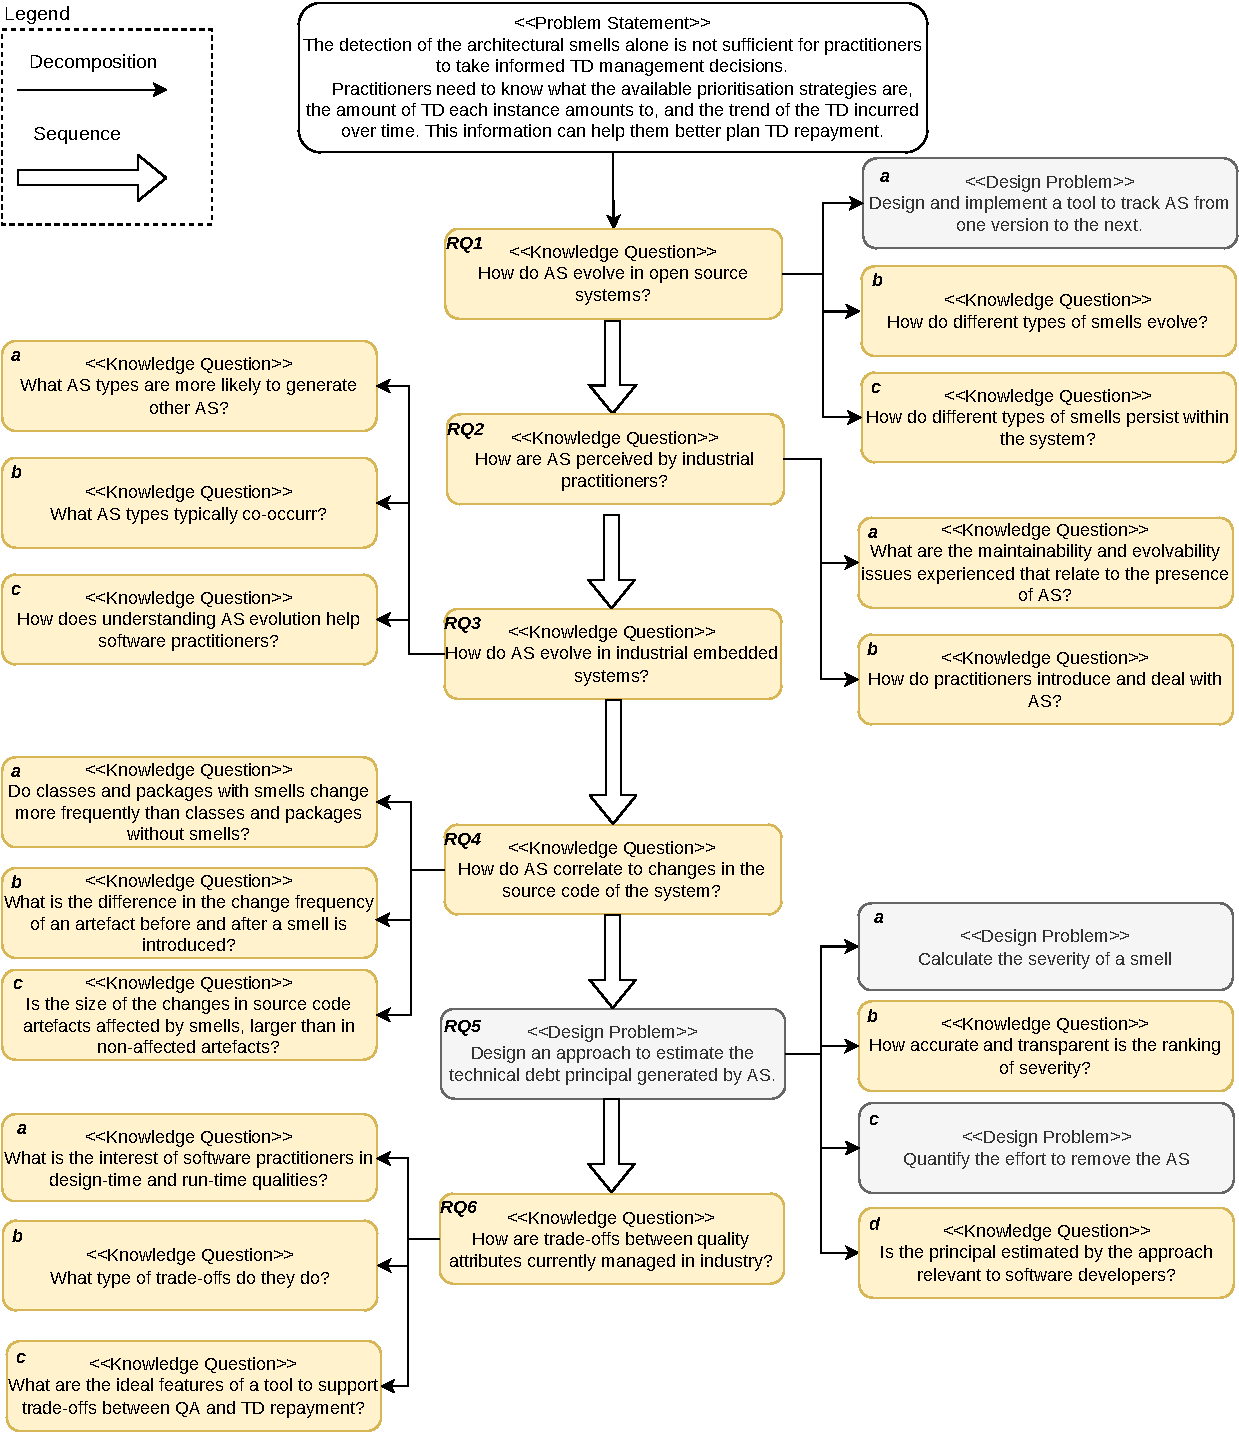
\includegraphics[width=\textwidth]{c1/problem-decomposition.pdf}
    \caption{The decomposition of the design problem tackled in this dissertation.}\label{fig:intro:problem-decomposition}
\end{figure}

The problem statement (see Figure \ref{fig:intro:problem-decomposition}) argues that practitioners cannot take informed decisions by relying on the detection of AS instances alone.
The smells detected also need to be quantified in terms of TD, prioritised, monitored and paid back in order for AS management to be effective.
Without support for these activities, the practitioners' ability to manage architectural TD is significantly limited, ultimately affecting the sustainability of the system.

As a first step towards addressing the stated problem, we decided to investigate how AS evolve in long-lived software systems, starting with open source systems. Thus we formulated RQ1: \textit{``How do AS evolve in open source systems?''} 
Answering RQ1 would allow to address the stated problem in two ways. First, obtaining an understanding of AS evolution can help researchers formulate general rules for prioritising AS based on their historical evolution.
Second, a better understanding of the evolution of a smell can help design a better approach to quantify the amount of TD incurred.
Studying the evolution of AS entails studying two aspects: the evolution of the individual AS instances (RQ1b) and the persistence of AS instances within the system (RQ1c). This study required analysing 524 releases belonging to 15 open source projects.
The tool \textsc{Arcan} was used to detect the architectural smells and a custom tool was designed and developed to track them from one release to the next (RQ1a).

One of the findings of RQ1 is that some smells may be the result of intentional design.
The investigation of RQ1, being a purely quantitative analysis based on the mining of software repositories, cannot provide any further insight on why practitioners intentionally introduce smells or whether they consider the consequences of doing so on software maintenance and evolution.
Moreover, since RQ1 focuses on open source projects only, it is hard to extend the findings to an industrial context.
Therefore, we formulated RQ2: \textit{``How are AS perceived by industrial practitioners?''}
The goal of RQ2 is two-fold: (1) understand the issues stemming from the presence of AS and that affect maintenance and evolution (RQ2a); and (2) explore how and why practitioners introduce and deal with AS (RQ2b). 
To answer RQ2, we designed a case study and interviewed 21 practitioners from 3 companies in Europe that work with both Java and C/C++.
The findings of RQ2 are particularly interesting for researchers as they can better understand the problems faced by practitioners and design solutions accordingly.

While investigating RQ2, practitioners admitted that, in most cases, 
smells are introduced inadvertently due to bad design decisions, and that their long-term effects would only manifest a long time (many months, or years) after the introduction.
This means, however, that other smells could be introduced in a component before severe maintenance issues arise, thus casting doubt on whether the issues reported by practitioners can be associated to a single smell or more.

%However, they could not pinpoint what types of smells are exactly introduced, whether there is more than one smell affecting the same components, and in what order these smells were introduced to begin with.
To investigate this aspect, we had to study the introduction and evolution of AS while also collecting feedback from the architects and engineers that developed the components affected by the smells.
Thus, we formulated RQ3 \textit{``How do AS evolve in industrial embedded systems?''}
This RQ focuses on the evolution of AS, similarly with RQ1, but has a completely different focus: the co-occurrence and introduction order of smells, taking into account also the experiences of practitioners.
The context of the study also changes, as RQ3 focuses on industrial systems written in C/C++ (rather than open source Java systems) belonging to a large multinational company.
Answering RQ3 allows us to understand if there exists any pattern that can predict the introduction of a smell given the presence of another and what practitioners think about specific AS instances (and their evolution).
This kind of information can be used to improve prioritisation decisions (e.g. address the component that is most likely to be affected next).

One of the main findings of RQ2 (that was also confirmed in RQ3) was that most of the interviewed practitioners were concerned about the frequency of change in affected components and the propagation of changes to other components due to the presence of smells. 
Practitioners reported that several components that were affected by smells necessitated frequent maintenance.
To further study this aspect, and ensure that their feedback was not just the result of confirmation bias\footnote{Confirmation bias is the tendency to interpret, favor, or recall information in a way that supports one's prior beliefs or values.}, we formulated RQ4: \textit{``How do AS correlate to changes in the source code of the system?''}
Answering this question can help in understanding if elements affected by architectural smells have a higher chance of changing than elements that are not affected by smells.
This in turns can shed some light into the relation between AS and the amount of interest paid by practitioners that decide to not repay the debt represented by smells.
Answering this RQ required investigating 27 Open Source projects, involving 360 years of total development and over 305 millions of lines of code.

Research questions from 1 through 4 focus on investigating the problem: they are \emph{knowledge questions} and answering them can support researchers in understanding how smells evolve, how they are perceived by practitioners, how they relate with changes in the source code of the system; ultimately, they allow us to understand how to prioritise, quantify, and monitor smells.
In contrast, RQ5 is a \emph{design problem} focusing on the solution: \textit{``Design an approach to estimate the technical debt principal generated by AS''}.
The output obtained from the previous RQs is used in RQ5 to design a solution to quantify the amount of technical debt principal generated by architectural smells.
In particular, we ranked a set of architectural smells instances based on the knowledge acquired from the previous RQs (and from the literature) and then trained a machine learning model that is able to rank (from most to least severe) individual architectural smell instances based on their severity.
Next, we designed an approach based on the machine learning model that estimates the amount of technical debt principal of each instance.
Finally, we set up a case study to validate our approach by interviewing 16 practitioners (from both the open source and industrial worlds) and gauge how far the output provided is a relevant and meaningful estimate of the TD principal incurred by a smell.

During the validation of the solution in RQ5, we discovered an interesting phenomenon: while practitioners understand and relate to the amount of TD principal, they often have to tolerate the existence ofTD, hence sacrificing maintainability, in favor of other qualities.
This means that TD management decisions are affected by other qualities as well, and to better understand the implications of these trade-offs we formulated RQ6: \textit{``How are trade-offs between quality attributes currently managed in industry?''}
The output of this research question can help practitioners make better trade-off decisions regarding the repayment of technical debt.
We investigated this RQ by setting up a case study where we performed both interviews and a focus group.
In particular, we interviewed 14 different practitioners and held a focus group with 7 participants.


\subsection{Mapping empirical methods to the RQs}
The previous section decomposed the problem statement into knowledge questions and design problems.
To answer each knowledge question we adopted a number of different empirical methods.
Table \ref{c1:tab:overview-methodology} lists the empirical methods that were used to answer each knowledge question, as well as the corresponding sections in this thesis elaborating on the respective study design.

\begin{table}[]
    \footnotesize
    \centering
    \caption{Empirical methods used to answer the knowledge questions.}
    \label{c1:tab:overview-methodology}
    \begin{tabular}{@{}lm{3.75cm}m{2.75cm}m{2cm}l@{}}
    \toprule
    \textbf{Code} & \textbf{Knowledge Question} & \textbf{Empirical}\newline \textbf{Method} & \textbf{Primary}\newline \textbf{Data} & \textbf{Described in} \\ \midrule
    RQ1 & \textit{How do AS evolve in open source systems?} & Case study & Quantitative & Section \ref{c2:sec:case-study} \\
    RQ2 & \textit{How are AS perceived by industrial practitioners?} & Case study,\newline Grounded Theory & Qualitative & Section \ref{c3:sec:case-study}  \\
    RQ3 & \textit{How do AS evolve in industrial embedded systems?} & Case study,\newline Grounded Theory & Quantitative \& Qualitative & Section \ref{c4:sec:case-study} \\
    RQ4 & \textit{How do AS correlate to changes in the source code of the system?} & Case study & Quantitative  & Section \ref{c5:sec:design} \\
    RQ5b & \textit{How accurate and transparent is the ranking of severity?} & Experiment & Quantitative & Section \ref{c6:fig:case-study-design-rq2}  \\ 
    RQ5d & \textit{Is the principal estimated by the approach relevant to software developers?} & Case study,\newline Grounded Theory & Qualitative & Section \ref{c6:fig:case-study-design-rq2}  \\ 
    RQ6 & \textit{How are trade-offs between quality attributes currently managed in industry?} & Case study,\newline Grounded Theory & Qualitative & Section \ref{c7:sec:case-study} \\ \bottomrule
    \end{tabular}
\end{table}

Specifically, the empirical methods adopted in this PhD project are the following:
\begin{description}
    \item[Case study] in software engineering is an empirical enquiry that investigates a contemporary phenomenon within its real-life context \cite{Yin2003}. In other words, it is used to increase the knowledge and bring about change in the phenomenon being studied \cite{Runeson2012}. Case studies were originally used primarily for exploratory purposes, but they can also be explanatory, descriptive, and improving.
    The exploratory case study is the main research method used in this dissertation.
    
    \item[Grounded theory] is an exploratory research method used to generate theories, mainly from qualitative data. It is one of the most important methods in the field of qualitative data analysis and it is used to increase the theoretical sensitivity of the researcher as the data analysis progresses. Grounded theory was particularly useful in this PhD project as it allowed us to formulate new hypotheses and theories starting from the qualitative data collected \cite{Glaser1968}.
    It is important to mention that Grounded Theory is a full research method describing several steps, including how data can be collected; however, in this thesis, only the qualitative data analysis part of Grounded Theory was used, namely the Constant Comparative Method according to \cite{Glaser2017}).
    
    \item[Experiments] allow to measure the effects of manipulating one variable on another variable \cite{Runeson2012}. For this reason, experiments are particularly suitable for establishing cause-effect relationships.
    In this PhD project, the experiment was used to determine the effects of architectural smell-related variables on the accuracy of a severity prediction model.
    
\end{description}

\subsection{Overview of this dissertation}
The main body of this dissertation consists of six chapters (Chapters \ref{chap:2} - \ref{chap:7}).
All chapters are based on papers published in peer-reviewed conferences and journals, except for Chapter \ref{chap:6}, which, at the moment of writing, is still under review in a peer-reviewed journal.

The PhD student was the first author and main contributor in all studies. The other authors were: (a) the supervisors; (b) a fellow PhD student from a different research group (Ilaria Pigazzini), who contributed to two studies by helping with data collection in one study, and both data collection and analysis in the other; (c) a software architect (Umut Uyumaz) from one of the companies that we collaborated with, who helped with the data collection.

Each chapter aims at answering one research question as presented in Section \ref{c1:sec:problem-decomposition} and briefly summarised in the following paragraphs.
Table \ref{c1:tab:outline} depicts where each chapter was published and the chapter number.
Finally, Chapter \ref{chap:8} concludes the dissertation by outlining the main results obtained from each empirical study and discusses future work opportunities.

\begin{table}[]
    \centering
    \caption{Outline of the studies of this dissertation.}
    \label{c1:tab:outline}
    \begin{tabular}{lm{6.5cm}lm{2cm}}
    \hline
    \textbf{Code} & \textbf{Research Question} & \textbf{Chapter} & \textbf{Published to} \\ \hline
    RQ1 & \textit{How do AS evolve in open source systems?} &  Chapter \ref{chap:2} & ICSME'19 \\
    RQ2 & \textit{How are AS perceived by industrial practitioners?} & Chapter \ref{chap:3} & IEEE Software \\
    RQ3 & \textit{How do AS evolve in industrial embedded systems?} &  Chapter \ref{chap:4} & EMSE \\
    RQ4 & \textit{How do AS correlate to changes in the source code of the system?} &  Chapter \ref{chap:5} & JSEP \\
    RQ5 & \textit{Design an approach to estimate the technical debt principal generated by AS} & Chapter \ref{chap:6} & Journal (under review) \\
    RQ6 & \textit{How are trade-offs between quality attributes currently managed in industry?} & Chapter \ref{chap:7} & SQJ \\ \hline
    \end{tabular}
    %{\footnotesize*Under review}
\end{table}

Chapter \ref{chap:2} is based on a paper published in the 2019 International Conference of Software Maintenance and Evolution (ICSME)(Sas, Avgeriou, Arcelli).
In the paper, we investigate the evolution of architectural smells in 14 open source Java systems.
In particular, we look at how their characteristics (or properties) evolve over time, and how long smells persist within the system. 

Chapter \ref{chap:3} is based on a study published in the IEEE Software magazine (Sas, Pigazzini, Avgeriou, and Arcelli 2020).
This paper aims at understanding how practitioners perceive the impact of architectural smells on their systems.
The specific goal is to allow researcher to better understand the practical maintenance issues faced by engineers when a system is affected by an architectural smell.
To do so, we interviewed 21 software practitioners from three different European companies and summarised their opinions on the matter.

Chapter \ref{chap:4} is an article published in the Empirical Software Engineering journal (EMSE) (Sas, Avgeriou, Uyumaz, 2022).
This paper features an empirical study where we analyse 9 C/C++ industrial projects, amounting to a total of 20 millions lines of code, and 38 releases for each project.
The goal of the study is two-fold: (1) investigate the evolution of architectural smells in C/C++ industrial projects; and (2) understand the opinions of the engineers on the findings of the first part.

Chapter \ref{chap:5} is based on an article published in the Journal of Software Evolution and Process (JSEP) (Sas, Avgeriou, Pigazzini, Arcelli, 2022).
This article investigates the relation between architectural smells and source code changes.
In particular, we analysed 31 Java systems and over 3900 commits in order to determine the existence of a correlation between the presence of an architectural smell and a higher change frequency than a non-affected component. 
We studied two different aspects of source code change: frequency and size.

Chapter \ref{chap:6} is based on a paper that is currently under review in a peer-reviewed journal.
In this paper, we aim at providing an approach to estimate the amount of technical debt principal generated by an architectural smell.
To do so, we developed a sophisticated approach to train a machine learning model that predicts the severity of an architectural smell, which is then used to estimate the principal.
To validate the approach, we interviewed 16 practitioners to understand whether the estimations provided by our approach are reasonable estimations of the amount of principal.

Chapter \ref{chap:7} is based on an article published in the Software Quality Journal (SQJ) (Sas, Avgeriou, 2020).
The paper investigates the quality attribute trade-offs performed by practitioners in the embedded systems industry.
Specifically, we looked at the trade-offs between run-time qualities (e.g. Availability) and design-time qualities (e.g. Maintainability).
To carry out the study, we performed two rounds of interviews and a focus group, with a total of 21 practitioners involved in the study.

